\chapter{Gaussian Comparisons}


\section{CGMT}
Setup (Review from last time)

Suppose we have $\{X_i\}$ generated from the following process, where $y_i \in \{-1, 1\}$, $|\xi| = 1$, $\sigma$ known.

$$X_i = y_i \xi + \sigma Z_i$$

It is helpful to also define a few additional constants. First, if we have $n$ samples and dimension $d$, let $\alpha = \frac{n}{d}$ and define $P(Y_i = 1) = r$. In this section, we are using a linear function as a separator of the form 


$$\text{sign}(\frac{X_i^Tw}{\sqrt{d}} + b)$$

The goal is to learn $w, b$ so that we can minimize the error of new samples generated from the same distribution. In other words, if $X_{new}, y_{new}$ are from the same process, the goal is to learn $w^*, B^*$ to minimize

\begin{align*}
    \xi_{gen} &= \P(y_{new} \ne \text{sign}\big(\frac{X_{new}^Tw^*}{\sqrt{d}} + b^*\big) \\
    &= rQ\frac{b+1}{\sigma\tau} + (1-r)Q\frac{q-b}{\sigma \tau}
\end{align*}

Note that we defined two more (very) useful constants above, 

$$\tau := \frac{||w^*||}{\sqrt{d}}$$

$$q := \frac{\xi^Tw^*}{\sqrt{d}}$$

and the function $Q$ is defined as 

$$Q(x) := \frac{1}{\sqrt{2\pi}}\int_{x}^\infty e^{-t^2/2}dt$$

To summarize from last class, for a given $\lambda, \ell()$, we want to find $w^*, b^*$ such that


$$w^*, b^* = \min_{w,b} \frac{1}{d}\sum_{i=1}^n \ell(\frac{x_i^Tw}{\sqrt{d}} + b; y_i) + \frac{\lambda ||w||^2}{2d}$$

The trick observed previously is that we can turn this into the following "minmax" problem.


\begin{align*}
    &\min_{w,b} \max_{u \in \mathbb{R}^n} \frac{1}{d}\sum_{i=1}^n u_i\Big(\frac{\xi^Tw}{\sqrt{d}} + \frac{\sigma Z_i^T w}{\sqrt{d}} + by_i\Big) - \frac{1}{d}\sum_{i=1}^n \ell^*(u_i) + \frac{\lambda||w||^2}{2d} \\
    = &\min_{w,b} \max_{u \in \mathbb{R}^n} \frac{\sigma}{d\sqrt{d}} u^TZw + 
    \underbrace{\frac{1}{d}\sum_{i=1}^n u_i\left(\frac{\xi^Tw}{\sqrt{d}} + by_i\right)- \frac{1}{d}\sum_{i=1}^n \ell^*(u_i) + \frac{\lambda||w||^2}{2d}}_{f \left( u,w \right)}
\end{align*}

Note that the last three terms are a function $f(w,u)$ that is convex with respect to $w$ while concave with respect to $u$. 
The first term is a coupling between $w$ and $u$ through the gaussian matrix $Z$,
We apply CGMT here to simplify this first term by considering the case of fixing $w$ and $u$ in turn.
We can rewrite this in the form 

\begin{equation}\label{eq:cgmt_form_optimization}
    \min_{w,b} \max_{u \in \mathbb{R}^n} \frac{\sigma}{d\sqrt{d}} ||u||s^Tw + \frac{\sigma}{d\sqrt{d}} ||w||u^Tg +
    f\left(u,w\right)
\end{equation}

Our goal is to solve \ref{eq:cgmt_form_optimization} for $w$ and $b$. 
However, since all the terms in the optimization ($\{u,w,b\}$) are high-dimensional vectors, this optimization is difficult. 
We thus proceed to try to reformulate this problem in terms of scalar optimization, based on our knowlege of the final quantities of interest (i.e. the norm of $w$ and inner product with $\xi$).
A useful "trick" is to add an additional minimization to the above problem, where we use $\tau = \frac{||w||}{\sqrt{d}}$ and $q = \frac{\xi^Tw}{\sqrt{d}}$. Adding this additional minimization simplifies the functional form significantly, to give

\begin{align}\label{eq:tau_q_optimization}
	\min_{\tau, q} \min_{\frac{||w||}{\sqrt{d}} =
	\tau, \frac{\xi^Tw}{\sqrt{d}} = q} \max_{u \in \mathbb{R}^n} \frac{\sigma||u||}{d\sqrt{d}} s^Tw + \frac{\sigma\tau}{d} u^Tg + 
	\frac{1}{d}u^T(q + by) - \frac{1}{d}\sum_{i=1}^n \ell^*(u_i) + \frac{\lambda\tau^2}{2}
\end{align}

Note that in \ref{eq:tau_q_optimization} the term $q$ in the inner product (with $u^T$) refers to a \textit{vector} whose entries are all $q$. 
Compare with \ref{eq:cgmt_form_optimization} for detail.
This was useful because now only the first term depends on $w$.

We now proceed to apply the min/max conditions.
With regard to first term, we (in an unconstrained setting) would like to align $w$ perpendicular to $s$ to minimize it. 
However, we cannot choose an arbitrary direction for $w$ since we are constrained by $q$.
To proceed, we can rewrite $s$:

\begin{equation}\label{eq:s_decomposition}
s = |s^T\xi|\xi + P_{\xi^{\perp}}(s)
\end{equation}

Note that this simply corresponds to decomposint $s$ into a direction parallel and perpendicular to $\xi$.

We now use \ref{eq:s_decomposition} to rewrite the first term of \ref{eq:tau_q_optimization}:

\begin{align*}
    s^Tw/\sqrt{d} &= \big(|s^T\xi|\xi + P_{\xi^{\perp}}(s) \big)\big(q\xi + P_{\xi^{\perp}}(w)/\sqrt{d}\big) \\
    &= qs^T\xi + P_{\xi^{\perp}}(s)^TP_{\xi^{\perp}}(w)/\sqrt{d} \\
    &= qs^T\xi - \sqrt{\tau^2 - q^2}\sqrt{(||s||^2 - (s^T\xi)^2)/d}
\end{align*}

The final line comes from noting that the total energy in the hyperplane orthogonal to $\xi$ must be $\sqrt{\tau^2-q^2}$. 
Further, since the vector $w$ is free within this hyperplane, we can choose to minimize the overall quantity by choosing it to lie parallel and in the opposite direction to  $P_{\xi^{\perp}}(s)$.
This is an \textit{exact solution} to the high dimensional optimization over $w$, allowing us to rewrite the problem \ref{eq:tau_q_optimization} as:

\begin{equation}\label{eq:reduced_dimension_optimization}
	\min_{\tau, q} \max_{u \in \mathbb{R}^n} 
	\frac{\sigma||u||}{d\sqrt{d}} \left(\underbrace{qs^T\xi}_{1} - \sqrt{\tau^2 - q^2}\sqrt{\underbrace{(||s||^2 - (s^T\xi)^2)/d}_{2}}  \right)+ 
	\frac{\sigma\tau}{d} u^Tg + 
	\frac{1}{d}u^T(q + by) - \frac{1}{d}\sum_{i=1}^n \ell^*(u_i) + \frac{\lambda\tau^2}{2}
\end{equation}

 Now we have not yet done anything probabilistic. However, we are looking in the case of when $d$ is large (high dimensional), therefore we can make a few helpful simplifications. 

 First, consider the term $1$ in \ref{eq:reduced_dimension_optimization}. 
 We can show this term is a small (approximately 0) perturbation in the high $d$ limit.
 This is becauseq $q$ is just a scalar, $s^T\xi$ is just a standard gaussian, so with high probability is order 1. Therefore, because we have a $\frac{1}{\sqrt{d}}$ coefficient in front of this, it goes to $0$ and we can remove this term.
 
 Consider term $2$ in \ref{eq:reduced_dimension_optimization}:
 
 $$\frac{||s||^2 - (s^T\xi)^2}{d} \longrightarrow 1$$
 
 This is because by the LLN (Law of large numbers), we have that
 
 $$\frac{||s||^2}{d} = \frac{\sum_{i=1}^d s_i^2}{d } = 1$$
 
 we can rigorously do this with error term and stochastic domination, but this is essentially $1$. The term $(s^T\xi)/d \longrightarrow 0$ by the same logic as above.
 
 
 Remember that we have the special case when: 
 
 
 $$\ell(x) = (x-1)^2$$ 
 
 $$\ell^*(u) = u^2/2 + u$$
  With these simplifications, we can rewrite our entire problem as the following.

 
 \begin{align*}
	 \min_{\tau, q} \max_{u} \frac{-\sigma||u||}{\sqrt{d}}\sqrt{\tau^2 - q^2} + \frac{1}{d}u^T(\sigma \tau g + q + by - 1) - \frac{1}{d}||u||^2 + \frac{\lambda\tau^2}{2}
 \end{align*}
 
 This problem looks much more promising, but we still have to deal with the $u$ vector which is still high dimensional. 
How can we simplify $u$? 
The nice thing is that $u$ appears as an inner product and as a norm in the expression, which is the same ``pattern'' that we observed for $w$. 
Thus, we apply the same idea as we used previously, by introducing an optimization over a new variable $\kappa \equiv\frac{||u||}{\sqrt{d}}$.
We now have:

\begin{equation}\label{eq:optimization_kappa}
	\min_{\tau, q} \max_{\kappa>0} -\sigma||u||\kappa\sqrt{\tau^2 - q^2} + 
	\underbrace{\frac{\kappa}{\sqrt{d}}\left|\left|\sigma \tau g + \left(q-1\right) + by \right|\right|}_{\star} -
	\frac{\kappa^2}{2} +
	\frac{\lambda\tau^2}{2}
\end{equation}

Note that the maximization in \ref{eq:optimization_kappa} is taken over positive $\kappa$ since it is a norm (and hence cannot be negative).

This is an elegant form for the problem, since we have reduced the problem to optimization over a low dimensional space (i.e. the scalars $\left\{ \tau, q, \kappa \right\}$).

To proceed with our analytical analysis, we would like to rewrite the term $\star$ in eq \ref{eq:optimization_kappa} by separating it into the sum of two orthogonal vectors (the vectors are orthogonal with high probability since we are working in high dimensions). 

\begin{equation}
	\begin{split}
		\star &= \frac{\kappa\sqrt{n}}{\sqrt{n}\sqrt{ d}} \sqrt{ \left| \left| \sigma\tau g \right| \right|^2 
	+ \left| \left| \left( q-1 \right) + by \right| \right|^2} \\
\end{split}
\end{equation}

We can simplify the first term here by noting that $ \left| \left| g \right| \right| /\sqrt{n} = 1$.

We can simplify the second term by noting that the norm should concentrate around the square root of the expectation value of its argument (since each coordinate is independently distributed).

\begin{equation}
\begin{split}
	\frac{ \left| \left| \left( q-1 \right) +by \right| \right|}{\sqrt{n}} 
	&\approx \sqrt{E \left( q-1 +by \right)^2} \\
	&= \sqrt{ r \left( q-1+b \right)^2 + \left( 1-r \right) \left( q-1-b \right)^2 }
\end{split}
\end{equation}

The second line follows by noting that $y$ can take on values of $\pm 1$ (they are the labels) with probability $r$ and $1-r$ respectively.

Putting everything so far together we have:

\begin{equation}\label{eq:optimization_expanded_b}
	\min_{\tau, q, b} \max_{\kappa>0} -\sigma\kappa\sqrt{\tau^2 - q^2} + 
	\kappa\sqrt{\alpha}\sqrt{\sigma^2\tau^2 +r \left( q-1+b \right)^2 + \left( 1-r \right) \left( q-1-b \right)^2 } + 
	\frac{\kappa^2}{2} +
	\frac{\lambda\tau^2}{2}
\end{equation}

The term $b$ in \ref{eq:optimization_expanded_b} is the \textit{bias} term in the linear classifier. 
We note that it appears only in quadratic form, so it can be optimized explicitly:

\begin{equation}\label{eq:optimal_b}
b^* = \left( 1-q \right) \left(2r-1  \right)
\end{equation}

Substituting this into \ref{eq:optimization_expanded_b} we have:

\begin{equation}\label{eq:optimization_tau_q_kappa}
	\min_{\tau, q } \max_{\kappa>0} -\sigma\kappa\sqrt{\tau^2 - q^2} + 
	\kappa\sqrt{\alpha}\sqrt{\sigma^2\tau^2 + 4 \left( 1-q \right)^2r \left( 1-r \right)}+ 
	\frac{\kappa^2}{2} +
	\frac{\lambda\tau^2}{2}
\end{equation}

\subsubsection{Maximization over $\kappa$}

We now proceed to optimize term by term, starting with $\kappa$. 
Again, we note that $\kappa$ appears (holding other variables fixed) as a quadratic equation, which can be solved explicitly for the maximum.
A slight complication arises because we have constrained $\kappa > 0$. 
If $\theta<0$ then the maximum of $\kappa$ will be found to be $<0$, so the constrained $\kappa \rightarrow 0$. 
See fig \ref{fig:analytic_optimal_kappa}. 

\begin{figure}
\begin{center}
	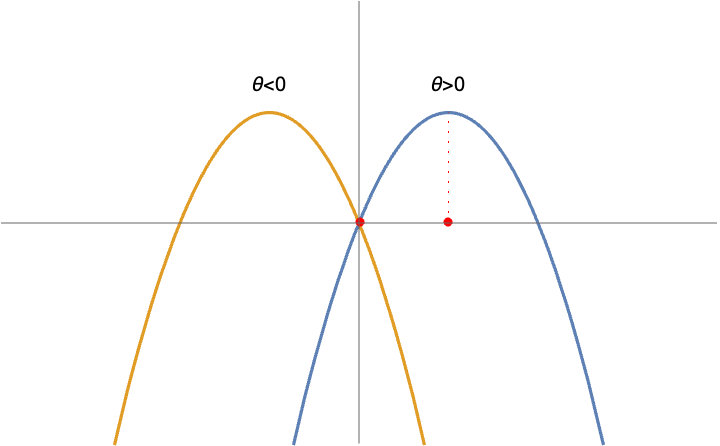
\includegraphics[scale=.5]{figures/twokappa.png}
\end{center}
\caption{Plot of $\kappa$ vs the optimization variable. The optimal values for $\kappa$ for the two regimes of $\theta$ are given by the red dots.}
\label{fig:analytic_optimal_kappa}
\end{figure}


We can now write (using a notation where $\vee$ is a notation for "if" i.e. it picks the \textit{larger} of its two arguments)

\begin{equation}\label{eq:optimal_tau_q}
	\min_{\tau, q }
	\frac{1}{2}\left[ 
	\underbrace{
		\sqrt{\alpha}\sqrt{\sigma^2\tau^2 + 4 \left( 1-q \right)^2r(1-r)}
	-\sigma\sqrt{\tau^2 - q^2}  }_{\star}
	\bigvee 0 \right]^2 + 
	\frac{\lambda\tau^2}{2}
\end{equation}

We have now reduced our problem to an optimization over two scalars. 

\textbf{Notes}
\begin{itemize}
	\item We recall that $\lambda$ controls the strength of regularization. 
(Note that if $\lambda = 0$ then this is a case of \textit{ridgeless} regression).
We take $\lambda \rightarrow 0^+$ so the problem tends to prefer solutions with minimal norm ($\tau$).
\item $\star$ is equivalent to the training loss. 
\item We see that if $\alpha <1$ (i.e. the number of data points is less than the dimension of the space) the training loss should be zero since there are more variables than equations in the linear classification (which can hence be perfectly fit). 
\end{itemize}

The final note can be illustrated by combining the constant terms in \ref{eq:tau_q_optimization} as c so we have:

\begin{equation*}
	\left[ \sqrt{\alpha}\sqrt{\tau^2 + \frac{1-q^2}{c}} - \sqrt{\tau^2 - q^2} \bigvee 0\right] ^2
\end{equation*}

In the case that $\alpha >0$ the first term dominates the second and a unique optimum for $\tau$ and $q$ can be found. 

In the case $\alpha <0$  the first term may be smaller than the second. Explicitly:

\begin{equation}\label{eq:alpha_less_than_0_inequality}
	\sqrt{\alpha}\sqrt{\tau^2 + \frac{1-q^2}{c}} < \sqrt{\tau^2 - q^2}
\end{equation}

This can be visualized as in \ref{fig:tau_q_solution}, which shows the region of 0 training loss as a function of $\tau$ and $q$. 
We note that this region is equivalent to the (degenerate) space of possible $w$ which give solutions to the underconstrained system of equations that form the linear regression problem.

\begin{figure}
\begin{center}
	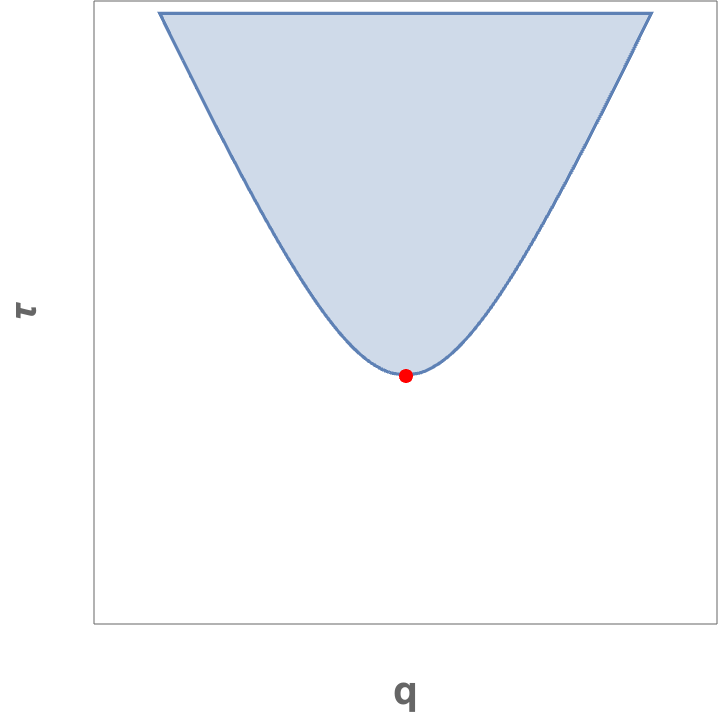
\includegraphics[scale=.5]{figures/tau_q_solution_region.png}
\end{center}
\caption{Plot of solution to inequality \ref{eq:alpha_less_than_0_inequality} as a function of $\tau$ and $q$. The minimal $\tau$ solution, which is picked out by the regularizer ($\frac{\lambda \tau^2}{2} $) corresponds to the tip of the parabola.}
\label{fig:tau_q_solution}
\end{figure}








